\section{Implications and Experimental Tests}

GCFT redefines physical ontology. Instead of particles and force carriers, it models all observable structure as tension patterns and resonance configurations in a single coherence field~$\Xi$. This perspective yields falsifiable predictions that diverge sharply from both quantum field theory and general relativity.

\subsection{No Need for Quantized Force Fields}

GCFT eliminates the need for separate quantum fields for each interaction. Electromagnetic, weak, strong, and gravitational effects all arise from internal structure within~$\Xi$:

\begin{itemize}
  \item \textbf{Phase gradients} ($\nabla \arg(\Xi)$): perceived as electric or gravitational acceleration.
  \item \textbf{Torsion harmonics} ($\nabla \times \nabla \arg(\Xi)$): encode magnetic interactions and binding stability.
  \item \textbf{Rupture thresholds}: manifest as transient field locks during topological transition events (e.g., bosons).
\end{itemize}

In this framework, what QFT interprets as exchange particles is simply the field’s response to coherence imbalance. There is no mediation — only resonance realignment.

\subsection{Mass Spectrum from Coherence Thresholds}

Mass in GCFT is not fundamental. It is the byproduct of how much luxion compression is required to maintain a stable phase-locked structure:

\begin{itemize}
  \item All rest mass originates from $\Xi$ compression and retention.
  \item Mass hierarchies emerge from knot topology and phase memory, not spontaneous symmetry breaking.
  \item Massless states, such as photons and gluons, remain below the coherence-lock threshold.
\end{itemize}

This explains not only the electron–muon mass gap, but also the quantized nature of meson families as tension modes of a shared coherence field.

\subsection{GCFT-Specific Predictions}

GCFT predicts several phenomena that do not arise in either the Standard Model or GR:

\begin{itemize}
  \item \textbf{Mass-gap inversion}: unexpected emergence of resonant structures at forbidden mass scales.
  \item \textbf{$\Xi$-chirps before decay}: phase-tension buildup preceding decoherence, visible as soft harmonics or spectral tails.
  \item \textbf{Composite state asymmetries}: mesons with unusual decay paths due to internal phase interference.
  \item \textbf{Recoil-based deformation patterns}: small-angle scattering anomalies from $\Xi$-field rebound, not momentum transfer.
\end{itemize}

These effects constitute clean falsifiability targets for future precision experiments.

\paragraph{Quantitative Coherence Thresholds and Timing Predictions.}
GCFT also yields testable quantitative predictions for coherence dynamics in high-energy and decay processes:

\begin{itemize}
  \item \textbf{Pre-decay $\Xi$-chirps}: Leptons and mesons (e.g., muon, kaon) should emit a transient soft-band coherence ripple prior to standard decay. Predicted duration $\tau_{\Xi} \sim 10^{-21}$~s; energy scale $\sim 10^{-2}$~eV. Detectable via high-resolution decay timing or spectral analysis in isolated environments.
  
  \item \textbf{Collider delay asymmetries}: W and Z boson production events should exhibit femtosecond-scale delay jitter caused by local coherence rupture and field rebalancing. These timing deviations would appear as stochastic scatter around expected SM lifetimes and may be detectable with ultrafast calorimetry at LHC or SHiP.
  
  \item \textbf{Mass–luxion scaling relation}: All stable particles obey the GCFT scaling law
  \[
  m = \frac{N_\text{lux} \cdot E_\text{lux}}{V},
  \]
  where $E_\text{lux} \sim 13.6$~eV and $V$ is the coherence confinement volume. This accounts for the observed lepton and hadron mass hierarchy without recourse to symmetry breaking or coupling constants.
\end{itemize}

These effects are falsifiable: the absence of coherence pre-signals, timing jitter, or systematic deviation from the predicted mass–volume relation in precision collider and decay data would challenge GCFT’s coherence field interpretation.


\subsection{Collider Signatures and Temporal Deviations}

Because GCFT structures retain memory and shape, high-energy collisions should reveal novel coherence-dependent signatures:

\begin{itemize}
  \item Measurable time delays in decay due to recoil-damping within $\Xi$.
  \item Angular asymmetries in baryon and meson scattering events.
  \item Suppressed or enhanced yields near phase transition thresholds.
  \item Low-frequency $\Xi$-chirps prior to decay in isolated or cold environments.
\end{itemize}

These signatures could be accessible to LHC, SHiP, or precision muon facilities using upgraded timing and calorimetry.

\subsection{\texorpdfstring{Time Crystal Behavior in Stable $\Xi$-Knots}{Time Crystal Behavior in Stable Xi-Knots}}

GCFT also predicts intrinsic time symmetry breaking. Certain stable $\Xi$-configurations — such as helium atoms — can enter persistent, self-organized oscillation states. These satisfy the criteria for time crystals~\cite{Wilczek2012}, yet arise without external forcing.

\begin{figure}[ht]
\centering
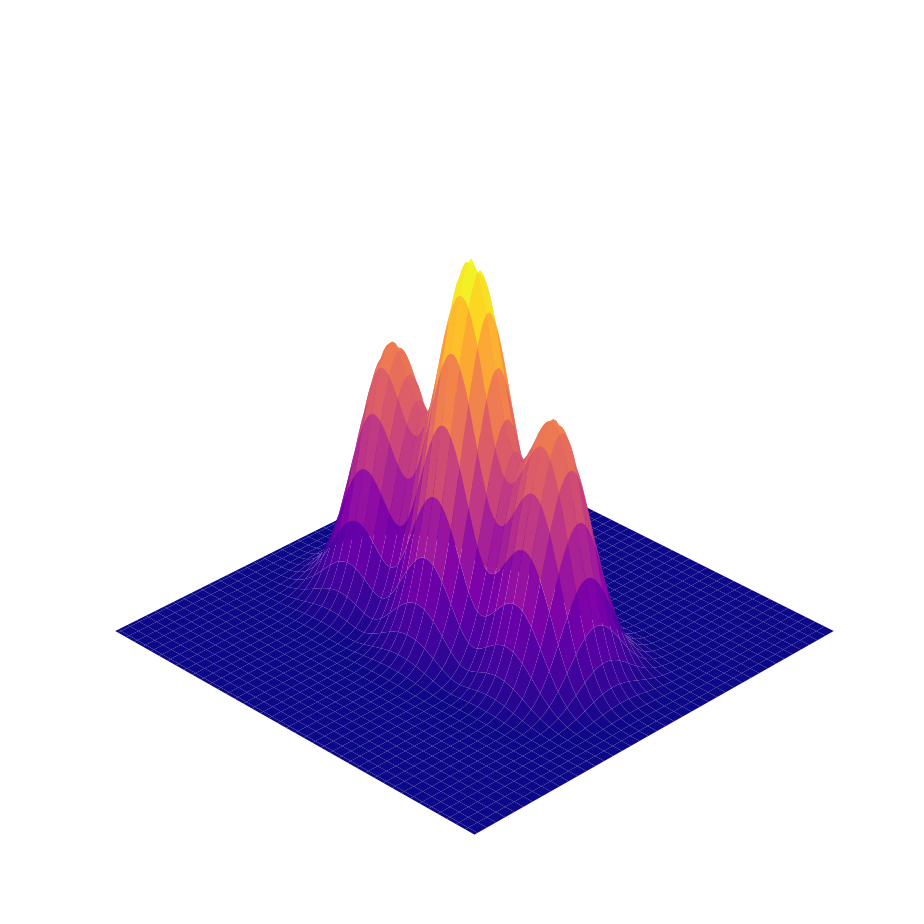
\includegraphics[width=0.48\textwidth]{figures/xi_time_crystal_3d_surface.png}
\caption{3D Simulation of a GCFT Time Crystal. A stable $\Xi$-knot forms around a central compression dome with two oscillatory lobes. The structure exhibits spontaneous phase oscillations over time, breaking time symmetry without external forcing.}
\label{fig:xi_time_crystal}
\end{figure}

\paragraph{Experimental Proposal: Helium as a Natural $\Xi$-Time Crystal}

In GCFT, the helium atom is modeled as a central compression node surrounded by two torsionally synchronized $\Xi$ lobes (electrons). This produces a coherent oscillation in internal phase geometry that breaks time symmetry spontaneously. When cryogenically isolated in high-coherence cavities, such atoms may reveal persistent torsional oscillations, energy level fluctuations, or field phase breathing—detectable through interferometry or low-noise spectroscopy. If observed, this would constitute the first naturally occurring mass-anchored time crystal, rooted not in Floquet engineering, but in field topology.

\subsection{Beyond the Standard Model — No Patchwork Required}

GCFT removes the need for many speculative extensions:

\begin{itemize}
  \item Supersymmetry is unnecessary — particle replication emerges from topology.
  \item GUTs are reframed as recursion patterns in $\Xi$ phase-space, not group mergers.
  \item Dark matter is reinterpreted as persistent coherence traps; dark energy as large-scale $\Xi$ drift.
  \item String theory is replaced by literal phase-string tension in continuous field space.
\end{itemize}

In this view, unification is not an addition — it is a collapse into one field.

\subsection{Conclusion}

The predictions above are distinct, falsifiable, and already partially supported by flyby anomalies~\cite{Hacquier2025a}, GW precursor chirps~\cite{Hacquier2025c}, and field stability in meson families. GCFT does not rely on hypothetical particles or unseen forces — only on the structure and behavior of a single field~$\Xi$, whose memory, timing, and curvature encode all that appears.

